
\section{Microcirculatory system}

The heart and larger arteries and veins are associated with the cardiovascular system, but those are only used for transportation of blood. Instead it is the capillaries, that permeate most tissues, that is responsible for the perfusion of tissue. These are the only vessels which permit exchange between the vessel and the surrounding interstitial fluids.  Factors that affect tissue perfusion is cardiac output, peripheral resistance and blood pressure. Capillaries are made not of single individual fluid conductors like veins and arteries, but instead formed into capillary beds. Here they work as a interconnected network of vessels.
As mentioned before the arteries decrease in size the further they expand into the peripheral system. The small arteries divide into arterioles which further divide into dozen of capillaries. The capillaries merge into a venule after the blood has been de-oxygenated. A capillary is divided into two segments, first the metarteriole and second the capillary. The blood flow between arterioles and venules can also be a direct connection, made by an arteriovenous anastomosis. This works as a bypass diverting blood flow around the capillary bed. An example of the structure of the capillary bed can be seen on \cref{fig:beds}.\cite{martini2012}
\begin{figure}[H]                                         
	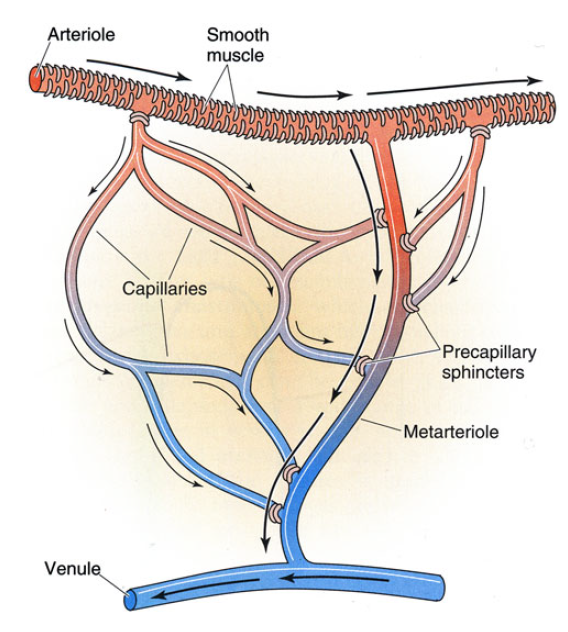
\includegraphics[width=.6\textwidth]{figures/capillary_bed}  
	\caption{The basic structure of a capillary bed, with arteriole on the left side of the bed and a venule on the right\cite{martini2012}.}
	\label{fig:beds}  
\end{figure}          

Each capillary entrance is controlled by a precapillary sphincter, which is composed of smooth muscle cells, that are able to contract or relax and thereby limit access of blood flow to certain capillaries. The blood flows relatively slow within the capillaries giving time for the two way exchange of nutrients and wastes. \cite{martini2012}

\subsection{Vasomotion}

The flow within the capillaries varies. This is among other thing due to the earlier mentioned precapillary sphincters opening and closing. The opening and closing of sphincters is part of the autoregulation process performed at a local level, to control the blood flow. The vascular system does not contain blood enough for every vessel a capillary beds to be filled with blood. Therefore only $25\%$ of the vessels in a capillary bed contains blood, and vessels activity needs to be well coordinated. Thermoregulation and control of nutrition balance are the primary functions of the microcirculatory system. Local changes in concentration of chemicals and interstitial fluids eg. dissolved oxygen concentrations in tissue modulates the vascular smooth muscles activity. Constriction and dilation of the vessel is thereby regulated by this periodic activity, also known as vasomotion. \cite{martini2012,geyer2004}

Under normal circumstances cardiac output remains stable and the control of local blood flow happens through local peripheral resistance within local tissues. The regulation of cardiovascular activity is controlled by local homeostatic mechanism. These make sure that demands such as oxygen and nutrients are meet and wastes are disposed.\cite{martini2012}

Physiological mechanism controlling vasomotion are not yet fully understood, but vascular smooth muscle activity has been shown to be roughly proportional to the tissue’s metabolic demand for oxygen.\cite{geyer2004} Studies also suggest that an increase in vasomotion activity enhances oxygen delivery\cite{goldman2001}. Further have some factors that trigger homeostatic mechanism to alter the vasomotion been said to have an impact. Factors that trigger dilation is called vasodilators and can be some of the following:\cite{martini2012,geyer2004}  
\begin{itemize}
	\item Decreased oxygen level or increased CO2 level
	\item Lactic acid or other acids generated from tissue cells
	\item Nitric oxide NO released from endothelial cells
	\item Rising concentrations of potassium ions or hydrogen ions in the interstitial fluid
	\item Chemicals released during local inflammation
	\item Elevated local temperature
\end{itemize} 

A vasodialation will result in increased oxygen, nitrients, buffers released to recreate homeostasis.
Factors that stimulate contriction is called vasoconstricters and can happen due to following:\cite{martini2012} 

\begin{itemize}
	\item Damaged tissue
	\item Aggregating platelets 
\end{itemize}

Furthermore mechanisms regulation vasomotion can be divided into three origins. These are endothelial/metabolic, myogenic and neurogenic. Endothelial regulation is based on registered O2, CO2, lactate, and H+ levels and from this releases nitric oxide as a vasodialater. Myogenic regulation senses strain and stress in vessels, which cause the smooth muscle to depolarize, contracting the vessels. Otherwise when the ion channels in the muscles close, the blood vessels relaxes leading to vasodialation. Neurogenic signals is said to come from the symphatic nervous system where these promote vasoconstriction.\cite{segal2005,ince2005,nilsson2003}


